\section{The LHCb detector}

The LHCb is one of four large experiments of the LHC at CERN. Its detector, a forward spectrometer, is located at one of the four interaction points.
There, mostly hadrons with a charm or bottom quark are studied.
The structure of the detector is shown in figure \ref{fig:lhcb} and its different components are briefly described in the following.

\begin{figure}[!htb]
  \centering
  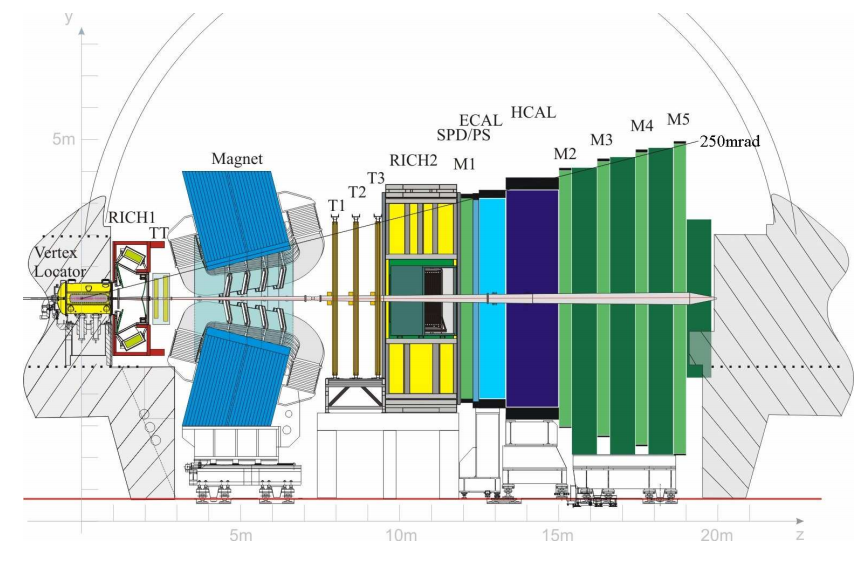
\includegraphics[width=0.8\textwidth]{graphics/lhcb.png}
  \caption{Components of the LHCb detector. \cite{lhcb}}
  \label{fig:lhcb}
\end{figure}

The Vertex Locator (VELO) tracks the trace of the particles after a collision. This way it is possible for the VELO to recontruct the position of the proton-proton collision: the primary vertex (PV).

The components TT, T1, T2 and T3 are four-layer silicon tracking detectors. They reconstruct the tracks of the particles after the collision. Furthermore T1-T3 contain tube modules filled with gas (Ar and $\text{CO}_2$). The crossing particles ionize the gas, which results in a signal.

Two magnets are used to measure the momenta of the particles. Due to the magnetic field the trace of the particles is curved and from the curvature the momenta of the particles can be determined. Because of existing systematic uncertainties up to 1\%, the polarity of the magnetic field is reversed from time to time.

For hadrons, the ring-imaging Cherenkov detectors (RICH1 and RICH2) differentiate between pions, kaons and protons. They contain gas or aerogel and due to the Cherenkov effect, the velocity of the crossing particles can be determined. This is possible since the angle of the emitted Cherenkov photons is related to the velocity of the particles.
Using the information about the particles' momenta and their velocities, the mass of the different particles (and therefore their flavour) can be computed.

A calorimeter system consisting of a scintillating pad (SPD), a preshower (PS) detector, an electromagnetic calorimeter (ECAL) and a hadronic calorimeter (HCAL) identifies the photons, electrons and hadrons. The particles deposit their energy in the different layers of the calorimeters. The photons are mainly absorbed in the ECAL, while hadrons are absorbed in the HCAL.
Only muons and neutrinos pass the calorimeters whithout being absorbed. Therefore muon chambers (M1-M5) are added to the detector to register muons.

Since there are plenty events happening at a high rate, the LHCb uses a trigger system to differentiate between potentially interesting events and other events. This trigger system consists of a hardware component and a software component. First, the hardware component uses information gathered from the calorimeters and from the muon chambers to decide whether an event is of interest. After that, the software component reconstructs the chosen events in real time and makes a decision whether the events are interesting for further analysis. If they are not considered to be useful, they are neglected.

\section{Theoretical foundations}
\label{sec:Theorie}

\subsection{The $B^0_s$ Decay}

In this analysis signal candidates for $B^0_s \rightarrow \psi(2S)K^0_S$ events, as shown in Figure \ref{fig:decay}, are extracted from a heavily polluted LHCb data sample.
The final-state mesons of the $B^0_s$ decay (the $\psi(2S)$ and the $K^0_S$) are not detected directly. Instead, the $\psi(2S)$ is reconstructed from two oppositely charged muons and the $K^0_S$ is reconstructed from two oppositely charged pions.

\begin{figure}[!htb]
  \centering
  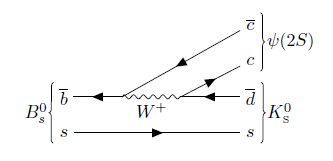
\includegraphics[width=0.5\textwidth]{graphics/decay.png}
  \caption{Leading order Feynman diagram of the decay $B^0_s \rightarrow \psi(2S)K^0_S$.}
  \label{fig:decay}
\end{figure}

A very similar decay is the $B^0 \rightarrow \psi(2S)K^0_S$ decay. Since it has the same final state as the $B^0_s$ decay and since it is also kinematically similar, it passes the same selection requirements as the $B^0_s$ decay.
Not only these decays, but also a combinatorial background can be found in the data sample. This combinatorial background stems from events coincidently passing the selection. For example if by chance two unrelated muons have a point of intersection, the algorithm will reconstruct them as a $\psi(2S)$, which then can be reconstructed to a false $B$ meson if combined with a $K^0_S$.

To differentiate the signals of the $B^0_s$ decay from the background a multivariate classifier is implemented.
